\documentclass[a4paper,11pt,hyperref]{ctexart}
\usepackage[left=3cm, right=3cm, top=2.5cm, bottom=2.5cm]{geometry}
\usepackage{graphicx}
\usepackage{amssymb}
\usepackage{bm}
\bibliographystyle{ieeetr}
\usepackage[ruled,linesnumbered]{algorithm2e}
\SetAlgoLined
\SetKwInput{KwIn}{输入}
\SetKwInput{KwOut}{输出}
\SetAlgorithmName{算法}{}{}

\title{\vspace{-5ex}\textbf{文献综述题目}\vspace{-5ex}}
\date{}

\begin{document}

\maketitle

\noindent\textbf{摘要:} 摘要内容

\noindent\textbf{关键词:} 关键词1,关键词2

\section{研究背景与意义}

\subsection{二级标题}

\subsection{二级标题}

\section{研究方向一}

\subsection{二级标题}

\subsubsection{三级标题}

\section{研究方向二}

\subsection{二级标题}

\subsubsection{三级标题}

\section{研究方向三}

\subsection{二级标题}

\subsubsection{三级标题}

\section{总结与展望}

\subsection{二级标题}

\subsection{二级标题}

\newpage

\section*{示例格式}

\subsection*{图片}
正文内容,参见图~\ref{fig1}。
\begin{figure}[h]
\centering
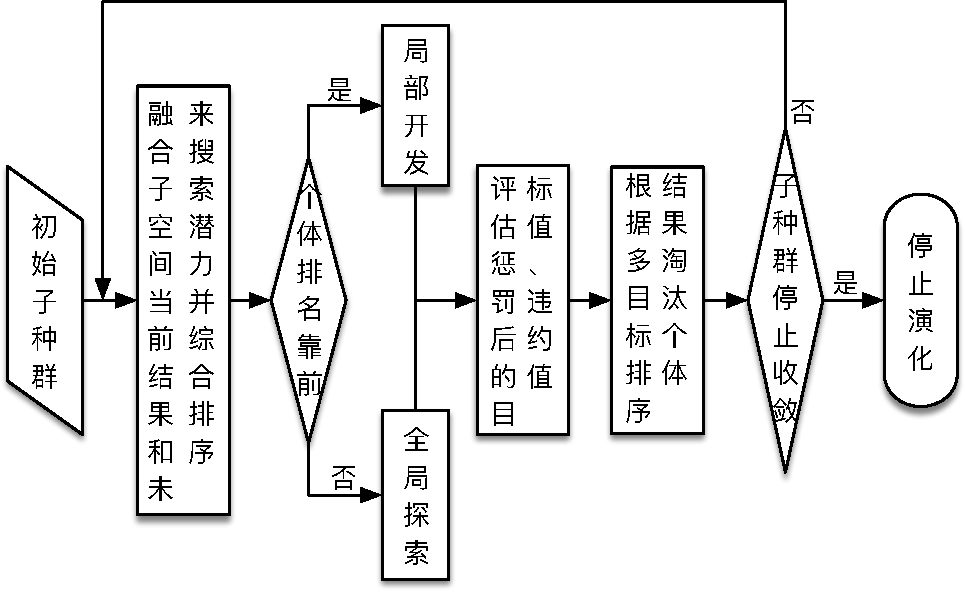
\includegraphics[width=0.65\textwidth]{fig1}
\caption{某某流程图}\label{fig1}
\end{figure}

\subsection*{表格}
正文内容,参见表~\ref{tab1}。
\begin{table}[h]
\centering
\caption{某某表}\label{tab1}
\begin{tabular}{l|cc}
  名称1 & 名称2 & 名称3 \\
  \hline
  A & 1 & 3\\
  B & 2 & 4
\end{tabular}
\end{table}

\subsection*{公式}
正文内容,如下:
\begin{equation}
	\label{equ1}
	\bm{v}'=\omega\bm{v}+\eta_1\bm{r}_1(\bm{x}_{lbest}-\bm{x})+\eta_2\bm{r}_2(\bm{x}_{gbest}-\bm{x})
\end{equation}
\begin{equation}
	\label{equ2}
	\bm{x}'=\bm{x}+\bm{v}'
\end{equation}
其中,$\bm{x}$和$\bm{x}'$分别表示移动前和移动后的位置,$\bm{v}$和$\bm{x}'$分别表示更新前和更新后的速度。

根据公式~\ref{equ1}和公式~\ref{equ2},得到

\subsection*{引用文献}
文献~\cite{Eiben1998evolutionary}~对目前演化算法领域在探索与开发方面的研究进行了综述。

 多目标优化算法的三个主要方向分别为基于~Pareto~排序的方法$^{\tiny\cite{Deb2002fast}}$、基于分解的方法、基于指标的方法。
\subsection*{算法}
正文内容,参见算法~\ref{alg1}
\begin{algorithm}[h]
  \KwIn{种群规模$N$,迭代次数$iters^{max}$,评估函数$f(\mathbf{x})$}
  \KwOut{最优解$\mathbf{x}_{best}$}
 初始化$\mathbb{P}:=\{\mathbf{p}_1,\cdots,\mathbf{p}_N\}$,$iters:=0$\;
  \While{$iters<iters^{max}$}{
    更新最优解\;
    归一化适应值\;
    \ForEach{$\mathbf{p}_i\in\mathbb{P}$}{
    \eIf{$f(\mathbf{p}_i) > 0.5$}{
    	局部开发\;
      }{
      全局探索\;
      }
      }
      $iters := iters + 1$
    }
  \caption{某某算法}\label{alg1}
\end{algorithm}


\newpage
\bibliography{reference}

\end{document}
